% Options for packages loaded elsewhere
\PassOptionsToPackage{unicode}{hyperref}
\PassOptionsToPackage{hyphens}{url}
%
\documentclass[
]{article}
\usepackage{lmodern}
\usepackage{amssymb,amsmath}
\usepackage{ifxetex,ifluatex}
\ifnum 0\ifxetex 1\fi\ifluatex 1\fi=0 % if pdftex
  \usepackage[T1]{fontenc}
  \usepackage[utf8]{inputenc}
  \usepackage{textcomp} % provide euro and other symbols
\else % if luatex or xetex
  \usepackage{unicode-math}
  \defaultfontfeatures{Scale=MatchLowercase}
  \defaultfontfeatures[\rmfamily]{Ligatures=TeX,Scale=1}
\fi
% Use upquote if available, for straight quotes in verbatim environments
\IfFileExists{upquote.sty}{\usepackage{upquote}}{}
\IfFileExists{microtype.sty}{% use microtype if available
  \usepackage[]{microtype}
  \UseMicrotypeSet[protrusion]{basicmath} % disable protrusion for tt fonts
}{}
\makeatletter
\@ifundefined{KOMAClassName}{% if non-KOMA class
  \IfFileExists{parskip.sty}{%
    \usepackage{parskip}
  }{% else
    \setlength{\parindent}{0pt}
    \setlength{\parskip}{6pt plus 2pt minus 1pt}}
}{% if KOMA class
  \KOMAoptions{parskip=half}}
\makeatother
\usepackage{xcolor}
\IfFileExists{xurl.sty}{\usepackage{xurl}}{} % add URL line breaks if available
\IfFileExists{bookmark.sty}{\usepackage{bookmark}}{\usepackage{hyperref}}
\hypersetup{
  pdftitle={Application User Guide},
  pdfauthor={Lance},
  hidelinks,
  pdfcreator={LaTeX via pandoc}}
\urlstyle{same} % disable monospaced font for URLs
\usepackage[margin=1in]{geometry}
\usepackage{graphicx,grffile}
\makeatletter
\def\maxwidth{\ifdim\Gin@nat@width>\linewidth\linewidth\else\Gin@nat@width\fi}
\def\maxheight{\ifdim\Gin@nat@height>\textheight\textheight\else\Gin@nat@height\fi}
\makeatother
% Scale images if necessary, so that they will not overflow the page
% margins by default, and it is still possible to overwrite the defaults
% using explicit options in \includegraphics[width, height, ...]{}
\setkeys{Gin}{width=\maxwidth,height=\maxheight,keepaspectratio}
% Set default figure placement to htbp
\makeatletter
\def\fps@figure{htbp}
\makeatother
\setlength{\emergencystretch}{3em} % prevent overfull lines
\providecommand{\tightlist}{%
  \setlength{\itemsep}{0pt}\setlength{\parskip}{0pt}}
\setcounter{secnumdepth}{-\maxdimen} % remove section numbering

\title{Application User Guide}
\author{Lance}
\date{25/04/2021}

\begin{document}
\maketitle

\hypertarget{application-user-guide}{%
\section{Application User Guide}\label{application-user-guide}}

\href{https://lanceteo89.shinyapps.io/INNOVAC/}{Application Link}

\hypertarget{layout}{%
\subsection{Layout}\label{layout}}

The application has 3 main sections:

\begin{enumerate}
\def\labelenumi{\arabic{enumi}.}
\tightlist
\item
  Top Navigation Bar
\item
  Side Panel
\item
  Main Panel
\end{enumerate}

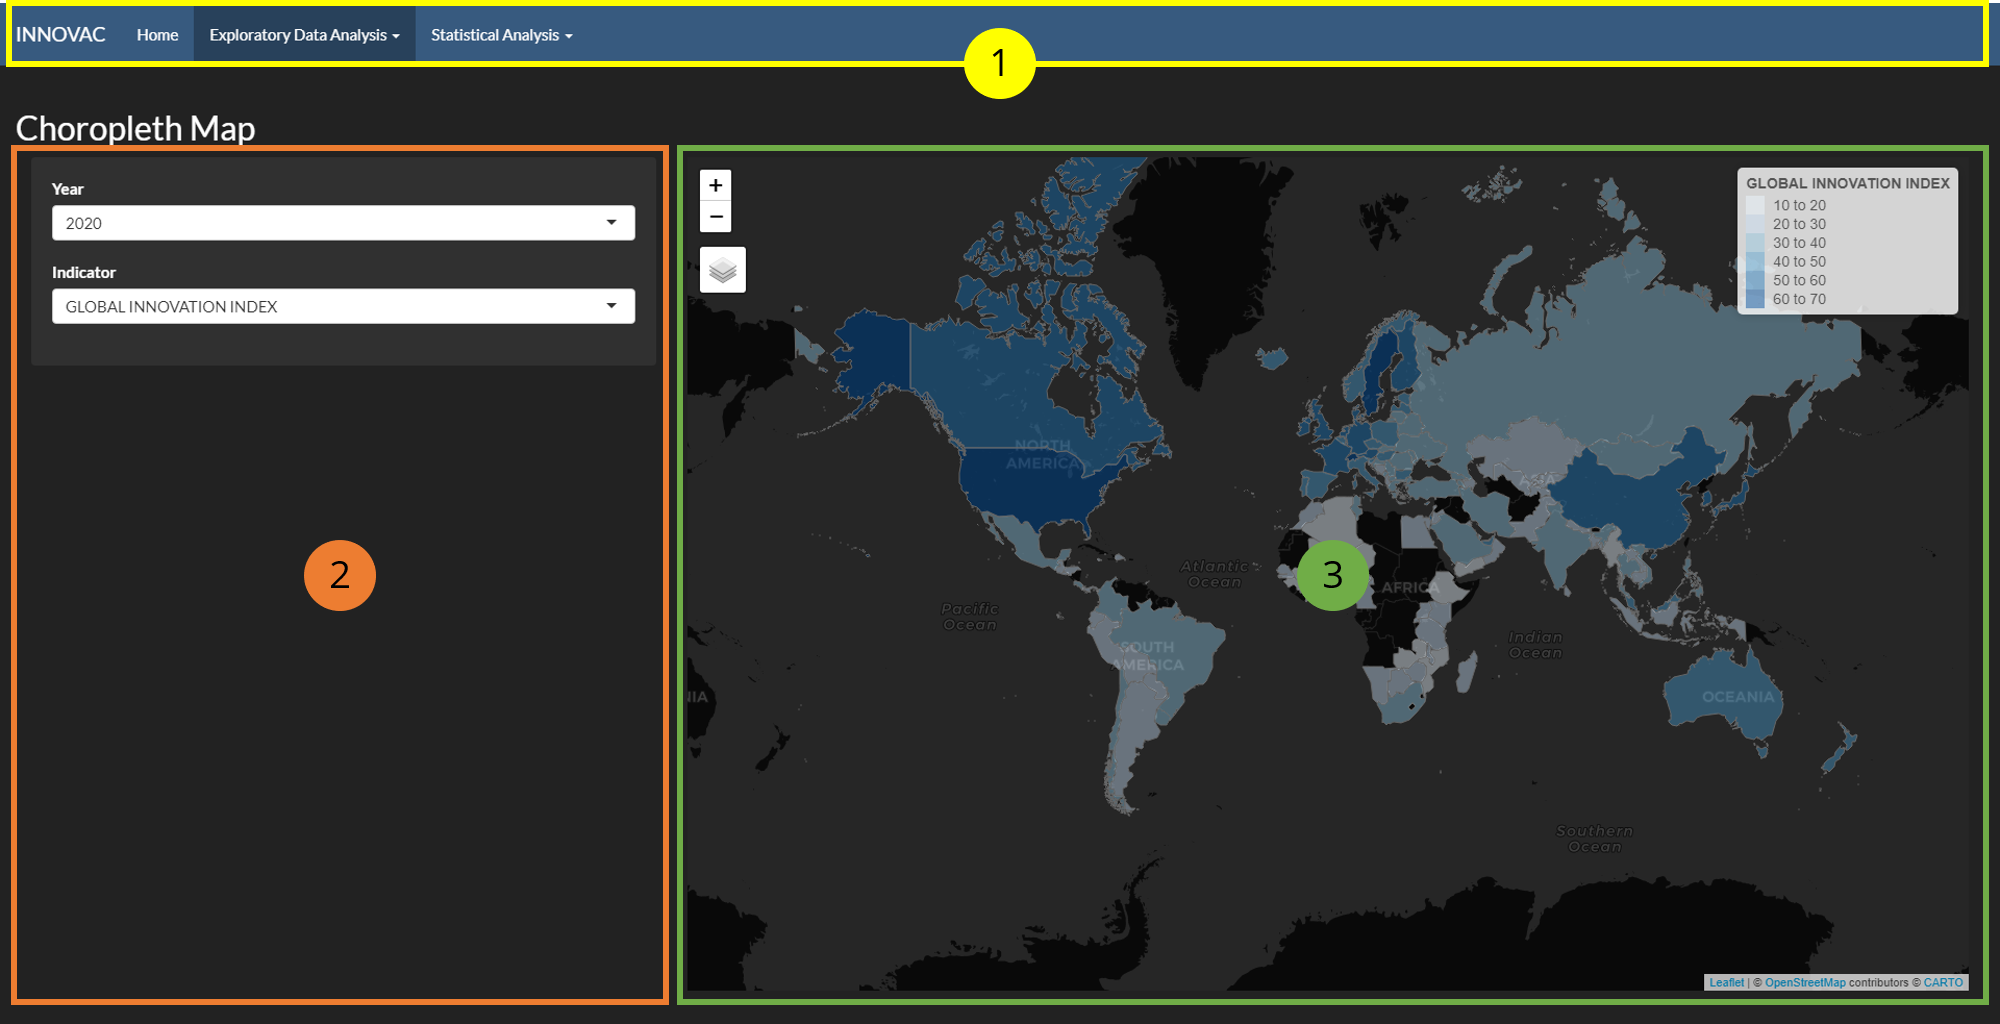
\includegraphics{./images/layout.png}

\hypertarget{top-navigation-bar}{%
\subsubsection{Top Navigation Bar}\label{top-navigation-bar}}

The top navigation bar has 2 main sections with drop-down selections:

\begin{enumerate}
\def\labelenumi{\arabic{enumi}.}
\item
  Exploratory Data Analysis

  \begin{itemize}
  \tightlist
  \item
    Choropleth Map
  \item
    Radar Chart
  \item
    Slope Graph
  \item
    Bubble Plot
  \end{itemize}
\item
  Statistical Analysis

  \begin{itemize}
  \tightlist
  \item
    Correlation Analysis
  \item
    Statistical Plots
  \item
    Hierarchical Clusting
  \end{itemize}
\end{enumerate}

\hypertarget{side-panel}{%
\subsubsection{Side Panel}\label{side-panel}}

The side panel provides the various toggling parameters for different
visualisation within the application. Some might come with brief
instructions on how to operation the application.

\hypertarget{main-panel}{%
\subsubsection{Main Panel}\label{main-panel}}

The main panel is where the visualisation will be shown.

\hypertarget{home---landing-page-of-the-application}{%
\subsection{Home - Landing Page of the
Application}\label{home---landing-page-of-the-application}}

The landing page introduces the motivation of the projects and outline
the contributors.

\hypertarget{exploratory-data-analysis}{%
\subsection{Exploratory Data Analysis}\label{exploratory-data-analysis}}

The \textbf{Exploratory Data Analysis} module provides users with
various tools to comb through the data and to obtain insights.

\hypertarget{choropleth-map}{%
\subsubsection{Choropleth Map}\label{choropleth-map}}

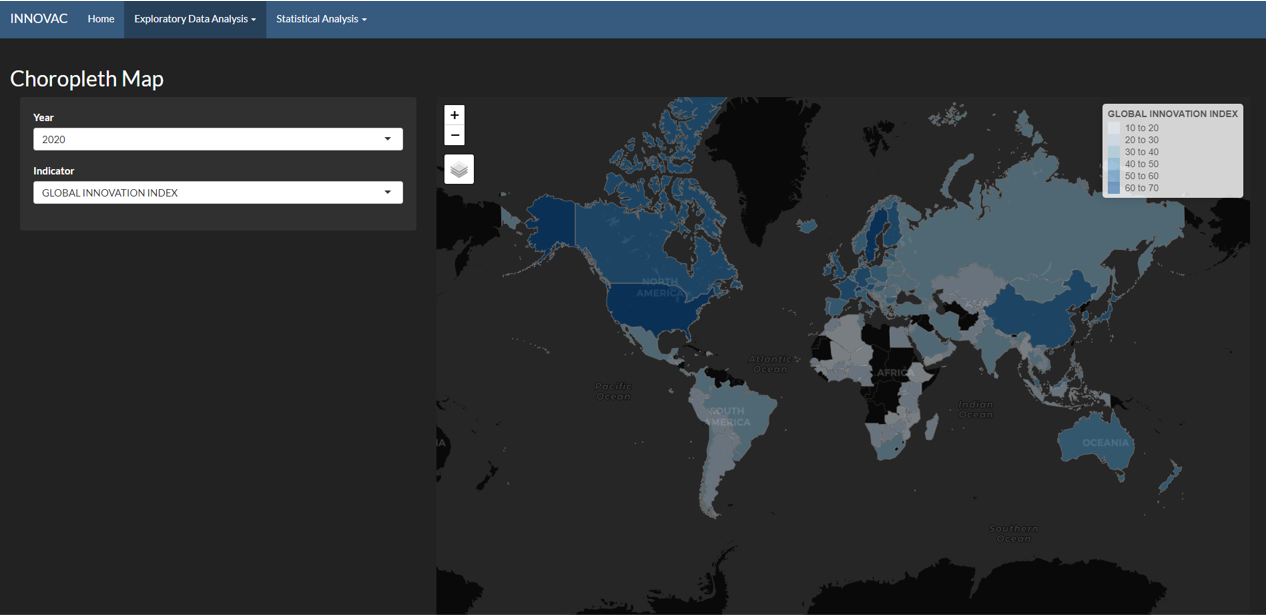
\includegraphics{./images/choropleth.png} The choropleth map provides a
board overview and the spread of different indicators across the
geospatial dimension. User can select the \textbf{Year} and
\textbf{Indicator} on the side panel to display on the world map.

The map is also interactive, hence, you will be able to zoom into the
country that you are looking for.

\hypertarget{radar-chart}{%
\subsubsection{Radar Chart}\label{radar-chart}}

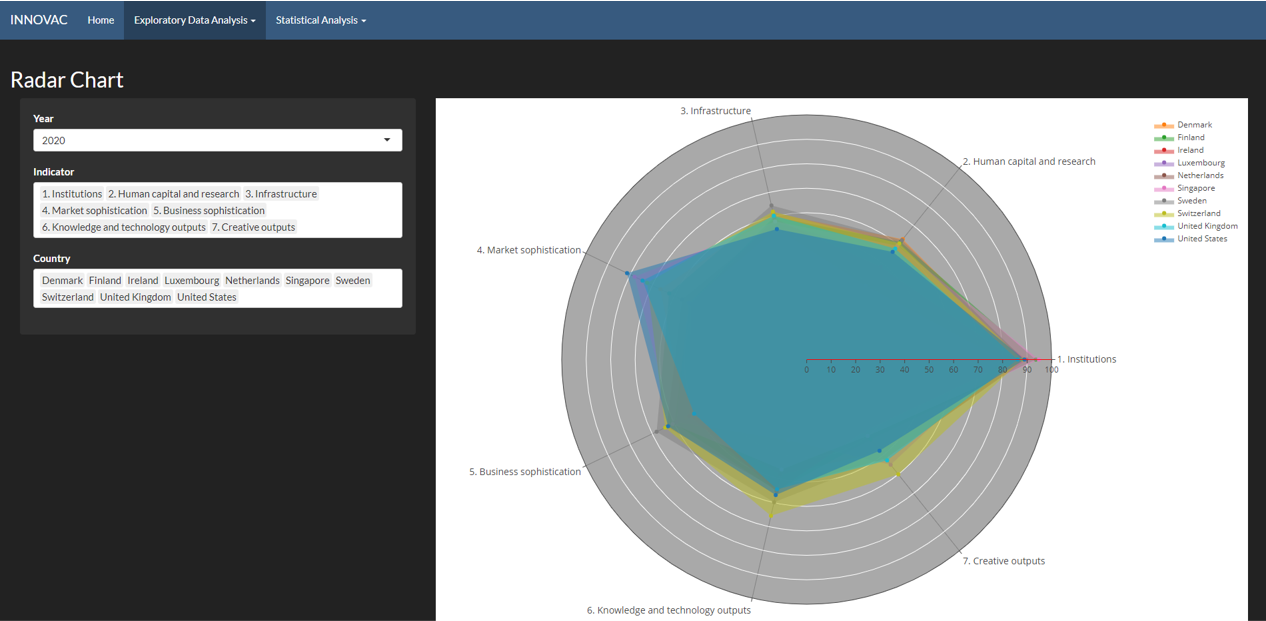
\includegraphics{./images/radar.png}

The radar chart provides a comparison between different selected
countries based on the selected set of indicators. User can select from
the side panel the \textbf{Year} of the data, the set of
\textbf{Indicators} to compare, and the different \textbf{Countries} to
compare among each other.

An overlay will be added for each country.

\hypertarget{slope-graph}{%
\subsubsection{Slope Graph}\label{slope-graph}}

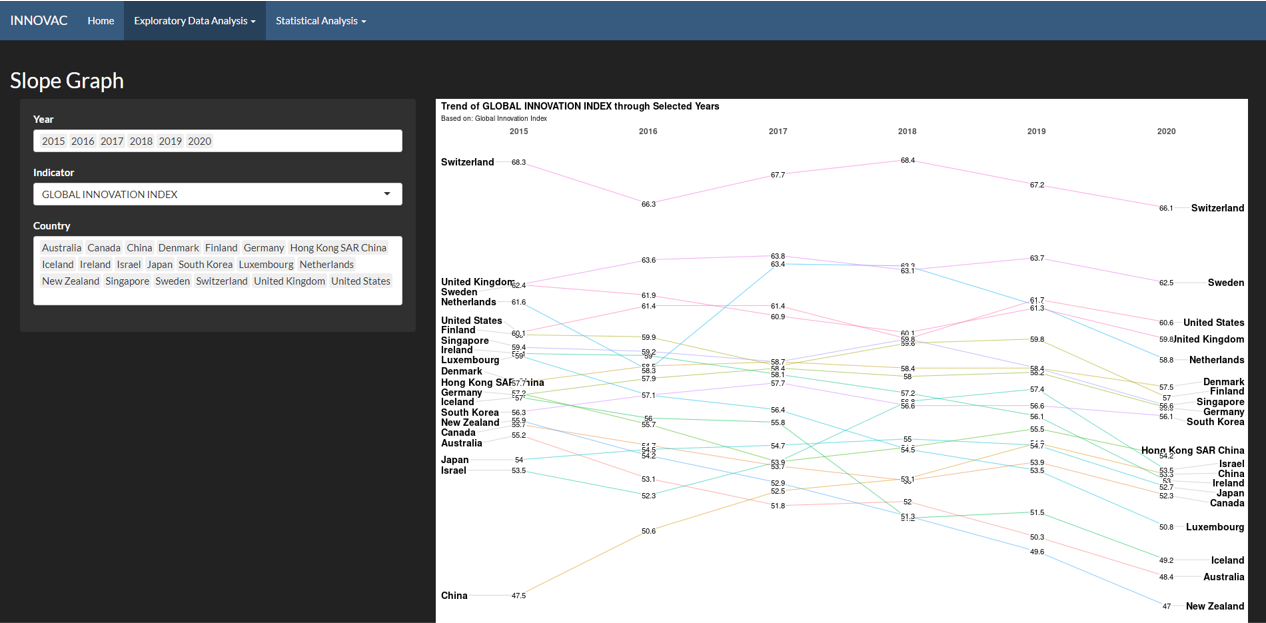
\includegraphics{./images/slope.png}

The slope graph provides a time-series analysis and comparison of the
selected indicator for select set of countries.

Users can select a range of \textbf{Year}, the \textbf{Indicator} to
trend, and the set of \textbf{Countries} to compare among each other via
the side panel.

\hypertarget{bubble-plot}{%
\subsubsection{Bubble Plot}\label{bubble-plot}}

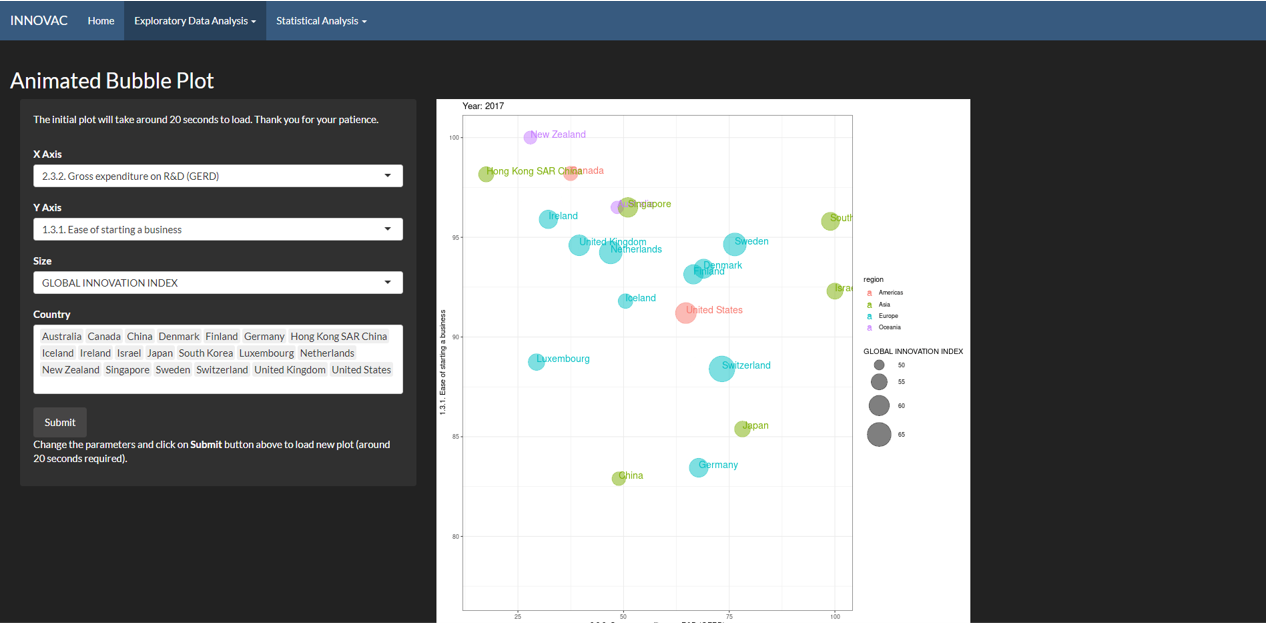
\includegraphics{./images/bubble.png} \emph{Note: the bubble plot is
animated and therefore, the initial plot and subsequent plot (via Submit
button) takes around 20 seconds to load}

The bubble plot provides the relationship between the 3 selected
indicators for each of the country. An animation is also added to look
at the changes for the 3 selected indicators across the years (from 2015
to 2020).

Users can choose an indicator for the 3 different parameters:
\textbf{X-Axis}, \textbf{Y-Axis}, and \textbf{Size} of the bubble, and
also choose the set of \textbf{Countries} to compare among each other.

\hypertarget{statistical-analysis}{%
\subsection{Statistical Analysis}\label{statistical-analysis}}

The \textbf{Statistical Analysis} module provides users with various
statistical techniques to deep dive into the dataset and uncovering
hidden patterns and trends.

\hypertarget{correlation-analysis}{%
\subsubsection{Correlation Analysis}\label{correlation-analysis}}

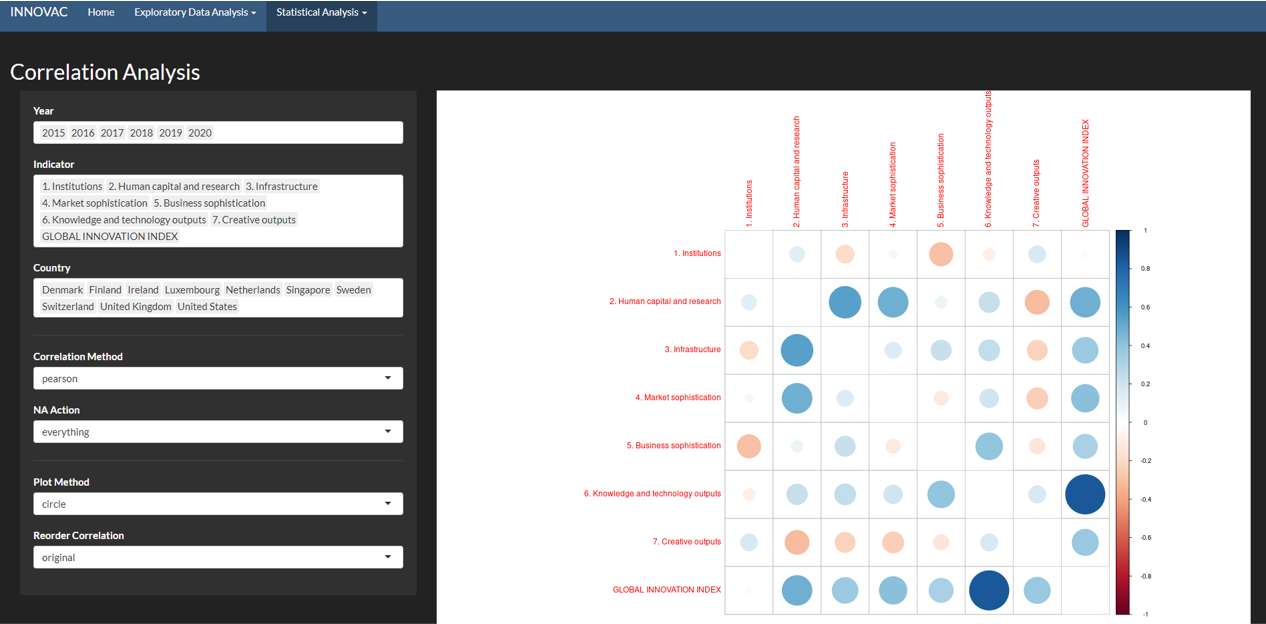
\includegraphics{./images/correlation.png} The correlation plot provides
users a measurement of the strength of association between the selected
set of indicators.

Users are able to select the \textbf{Year}, the set of
\textbf{Indicators} to correlate, filter the \textbf{Countries}, change
the \textbf{Correlation Method}, the way NA is handles via \textbf{NA
Actions}, the \textbf{Plot Method} and how the correlation is orders via
\textbf{Reorder Correlation}.

\hypertarget{statistical-plots}{%
\subsubsection{Statistical Plots}\label{statistical-plots}}

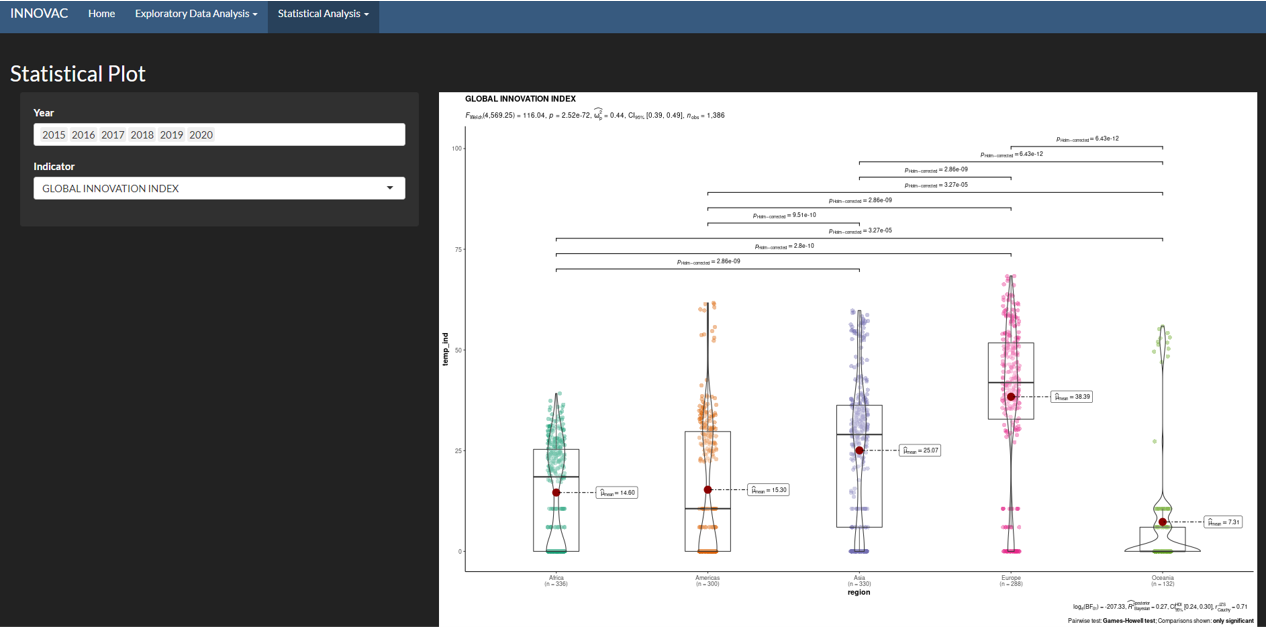
\includegraphics{./images/stats.png}

The statistical plots provides users with relevant statistical details
via a combination of a scatter plot, box plot, and a violin plot. The
plot is also \emph{publication-ready} courtesy of the \emph{ggstatsplot}
library.

Users are able to select the different \textbf{Years} and the
\textbf{Indicator} to compare among the different regions.

\hypertarget{hierarchical-clustering}{%
\subsubsection{Hierarchical Clustering}\label{hierarchical-clustering}}

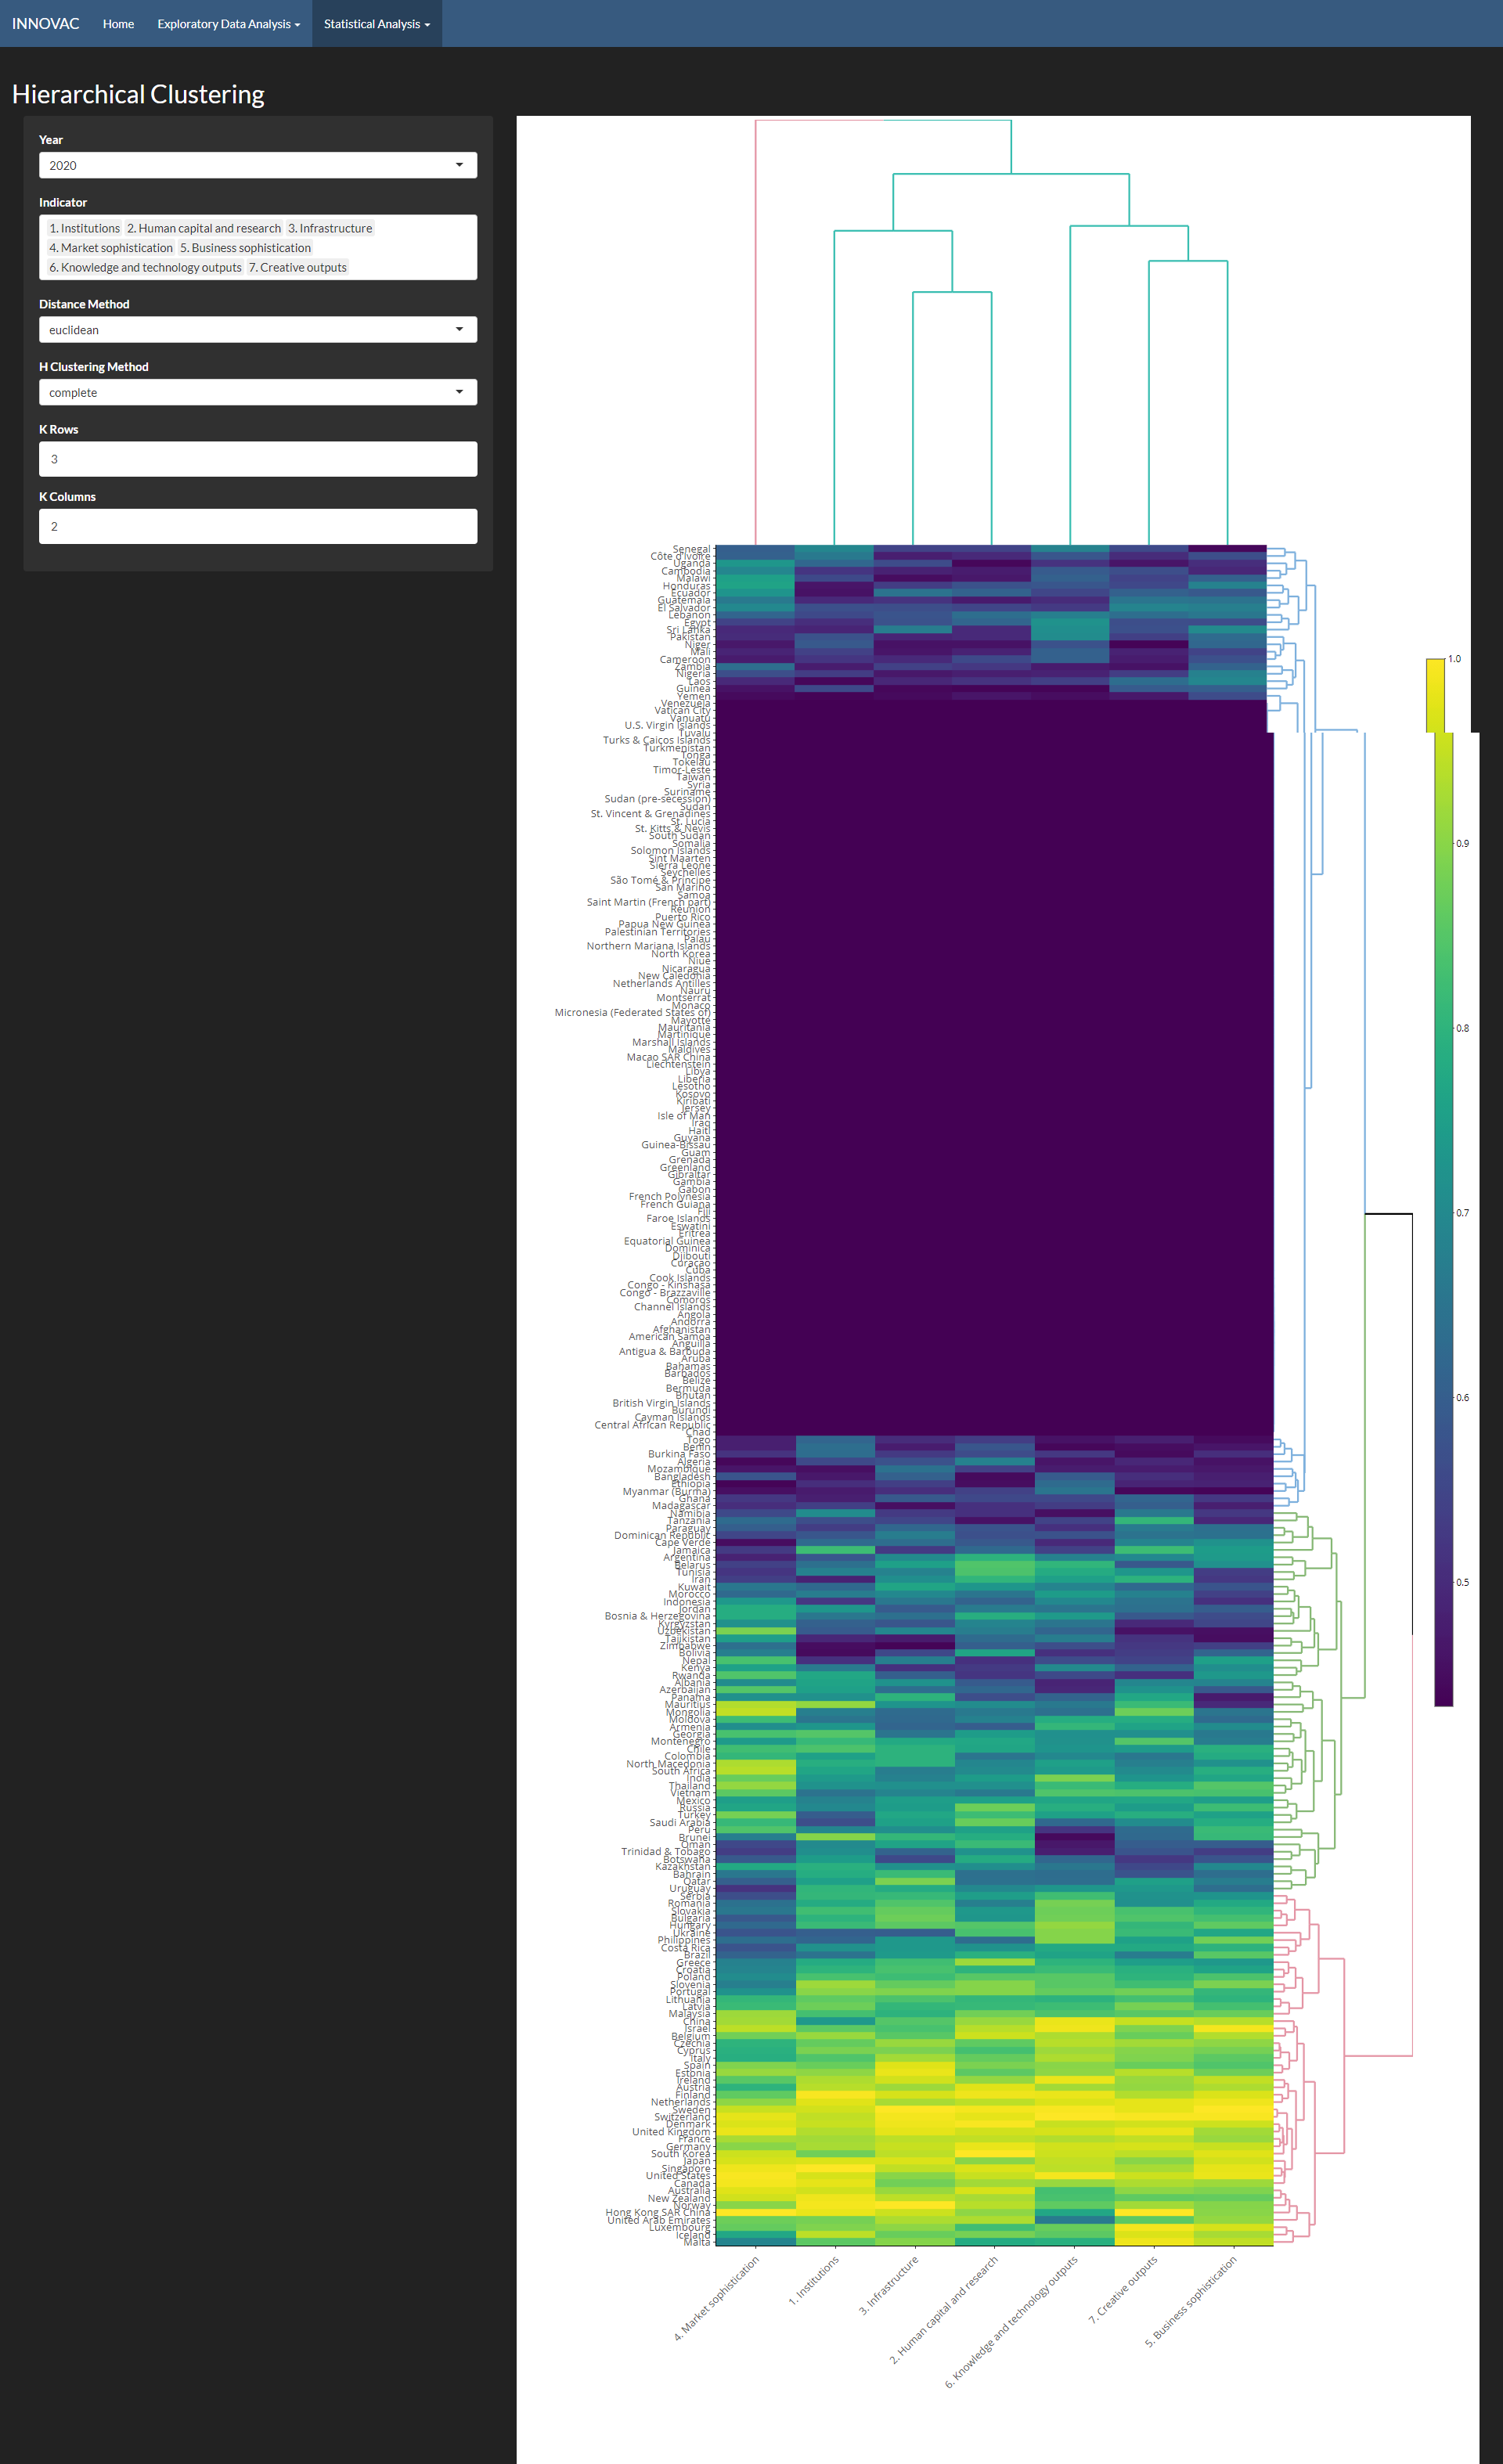
\includegraphics{./images/hclust.png} Hierarchical Clustering allows
users to cluster similar countries together via the selected indicator
in the selected year.

Users are able to select the \textbf{Year} of interest, the set of
\textbf{Indicators} for clustering, the \textbf{Distance Method} used,
the \textbf{Hierarchical Clustering Method}, the number of
\textbf{Clusters} for the countries and indicators.

\end{document}
